% Chapter 1

\chapter{Estado del arte} % Main chapter title

\label{Chapter1} % For referencing the chapter elsewhere, use \ref{Chapter1} 

\lhead{Capítulo 2. \emph{Estado del arte}} % This is for the header on each page - perhaps a shortened title
\section{Nomenclatura y definiciones previas}
En este documento llamaremos \emph{texto} a una secuencia de caracteres de un alfabeto finito {\it A} sobre la cuál se desea encontrar todas las ocurrencias de una o más secuencias de caracteres del mismo alfabeto, a las que llamaremos \emph{patrones}. Denotamos con {\it T} al texto, mientras que los patrones los representaremos con la letra {\it p} (en caso de ser uno solo) o $p_{i}$ (para referirnos al patrón i-ésimo de un conjunto ordenado de patrones). Denotamos con $\lambda$ una secuencia vacía, 
se consideran tanto {\it T}, {\it p} como $p_{i}$ , distintas de $\lambda$. A su vez nos referiremos a una entrada $k$ (el elemento $k$-ésimo desde el inicio de la secuencia) de una secuencia de caracteres $x$ mediante $x[k]$; definimos $x[k]=\lambda$ si $k$ es mayor que el largo de $x$. Los largos de las cadenas {\it T} y {\it p} se denotarán como $n$ y $m$ o $\mid T \mid$ y $\mid p \mid$ respectivamente, en caso de tener un conjunto de patrones, se denotará al largo del patrón $i$-ésimo como $m_{i}$ o $\mid p_{i} \mid$. Se notarán sub-cadenas que comiencen en la posición $i$ y finalicen en $j$ como $T[i,j]$ o $p[i,j]$.\\
Usaremos las nociones de izquierda y derecha en analogía con la escritura de textos en idioma castellano. Así diremos que $T[k]$ está a la izquierda de $T[k+1]$ y a la derecha de $T[k-1]$.\\
Dadas dos secuencias de caracteres $s$ y $t$, de largos $k$ y $j$ respectivamente, diremos que $t$ es \emph{sufijo} de $s$ si $s[k + 1 -j,k]=t$, si además se cumple que $j<k$ diremos que $t$ es \emph{sufijo propio} de $s$. Por otro lado diremos que $t$ es \emph{prefijo} de $s$ si $s[1,j]=t$, si además se cumple que $j<k$ diremos que $t$ es \emph{prefijo propio}.
\section{Algoritmos de búsqueda de un único patrón en un texto}
\label{sec:unpatron}
Los algoritmos que se presentan a continuación tienen como entrada un texto {\it T} sobre el cual se desea encontrar todas las ocurrencias de un único patrón {\it p}.\\
Algunos de los algoritmos que resuelven el problema planteado son: 
\begin{itemize}
\item Fuerza bruta
\item Rabin – Karp 
\item Knuth – Morris – Pratt (KMP) 
\item Boyer – Moore (BM)
\item Bitap 
\end{itemize}
En este documento se presentarán los algoritmos de fuerza bruta, KMP, BM y el uso de árboles de sufijo en la búsqueda de patrones. Estos algoritmos usan herramientas similares a los de AC y MSW que fueron evaluados experimentalmente en este proyecto. La evaluación de otros algoritmos como Rabin-Karp \cite{KARP} y Bitap \cite{BAEZA} queda como trabajo futuro.
\subsection{Algoritmo de fuerza bruta}
A la hora de resolver el problema de encontrar un único patrón dentro de una secuencia de caracteres, la primera idea que surge es realizar un algoritmo de fuerza bruta.\\
Este algoritmo consiste en hacer una recorrida secuencial sobre {\it T}, comparándolo carácter a carácter con el patrón de búsqueda {\it p} hasta que, o bien ocurra una diferencia o bien el patrón o el texto se hayan recorrido completamente. Al ocurrir una diferencia, se desplaza {\it p} una posición hacia la derecha (en relación al texto) y se comienza nuevamente con las comparaciones.\\
El tiempo de ejecución del algoritmo de fuerza bruta tiene un orden de ejecución de {\it mn} en el peor caso, siendo $\mid T \mid= n$ y $\mid p \mid = m$ ya que en cada posición $k$ del texto que cumpla que $k –  n \leq m$ se pueden llegar a ejecutar tantas comparaciones como el largo de {\it p}. La ventaja que presenta este algoritmo es su simpleza a la hora de implementarlo \\
\begin{example*}
En la figura \ref{fig:FuerzaBruta} se presenta un ejemplo de ejecución de este algoritmo, donde las celdas coloreadas en verde indican coincidencia, las grises que no se han realizado comparaciones y las rojas que se han encontrado diferencias.
\begin{figure}[H]
	\centering
		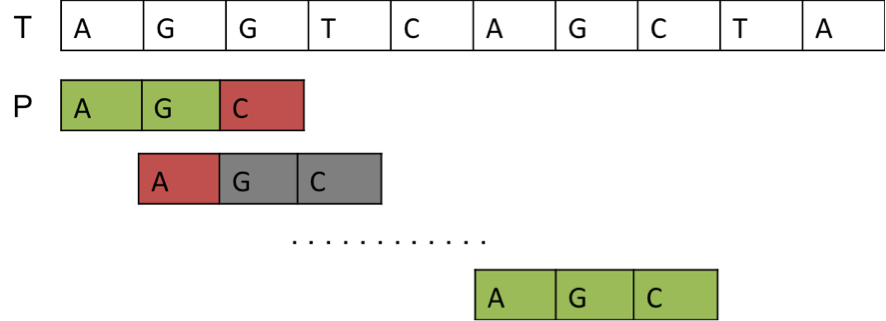
\includegraphics[scale=0.5]{Fuerza_Bruta.png}
		\rule{35em}{0.5pt}
	\caption[Ejemplo del algoritmo de fuerza bruta]{Ejemplo del algoritmo de fuerza bruta}
	\label{fig:FuerzaBruta}
\end{figure}
\end{example*}
\newcommand{\myrule} [3] []{
    \begin{center}
        \begin{tikzpicture}
            \draw[#2-#3, ultra thick, #1] (0,0) to (0.5\linewidth,0);
        \end{tikzpicture}
    \end{center}
}
\myrule{}{}
\subsection{Knuth Morris Pratt (KMP)}
\label{subsec:kmp}
El primer algoritmo que mejoró el orden de ejecución fue presentado por primera vez en junio de 1977 por Donald E. Knuth, James H. Morris y Vaughan R. Pratt \cite{KMP}.\\
A diferencia del algoritmo de fuerza bruta, KMP presenta la idea de saltar una secuencia de caracteres al ocurrir una diferencia ({\it missmatch}) entre un carácter del texto ({\it T}) y otro de {\it p} que se estén comparando.\\
Los autores de este algoritmo proponen realizar dos fases. En la primera se realiza la construcción de una tabla que indica cuántos caracteres se debe desplazar {\it p} con respecto al texto al ocurrir un fallo en la búsqueda. En la segunda fase se realiza una recorrida secuencial sobre el texto, comparando cada entrada con {\it p}. En caso de ocurrir un fallo se utiliza la tabla construida en la primera fase para conocer el desplazamiento que se debe realizar, en caso contrario se continua avanzando secuencialmente. Si se comparan con éxito los $m$ elementos de {\it p} con una sub secuencia del texto se tendrá una ocurrencia de {\it p} en el texto.
Este mecanismo permite evitar comparaciones que se sabe de ante mano serán inútiles, mejorando de esta forma el rendimiento de la búsqueda en comparación al algoritmo de fuerza bruta.\\
Para cada posición $i$, $i \leq \mid p \mid$, en el patrón {\it p}, definimos $sp_{i}'$ como el largo del sufijo más largo de $p[1..i]$ que es prefijo de {\it p} y además cumple que los caracteres $p[i+1]$ y $p[sp_{i}' + 1]$ son diferentes \cite{GUS}. 
\begin{example*}
Si consideramos $p = accgtacct$ se tiene que $sp_{1}' = sp_{2}' = sp_{3}' = sp_{4}' = sp_{5}' = 0$, $sp_{6}' = sp_{7} = 1$, $sp_{8}' = 3$.
\end{example*}
\myrule{}{}
Este algoritmo permite encontrar todas las ocurrencias de {\it p} en un {\it T} en $O(m+n)$.\\
Si consideramos $sp_{i}'$ como la función de fallos mencionada anteriormente, se puede definir el desplazamiento del algoritmo KMP en caso de fallos en términos de $sp_{i}'$. Dada una alineación de {\it p} y el texto, si ocurre un fallo en la comparación en la posición $i + 1$ respecto a {\it p} y $k$ respecto del texto, se debe desplazar el patrón $i - sp_{i}'$ posiciones hacia la derecha. De esta forma se tiene que $p[1,sp_{i}']$ se alinéa con $T[k-sp_{i}',k-1]$. Si una ocurrencia de {\it p} es encontrada en el texto se desplaza al patrón $m-sp_{m}'$ lugares.
\begin{example*}
Tomando $p = accgtacct$ y $T = accgtatttg$ se tiene que el algoritmo KMP al procesar el texto encuentra un fallo en la posición 7 ($i=6$). Como $sp_{6}' = 1$, el algoritmo KMP debe desplazar 5 posiciones a {\it p}. En la figura \ref{fig:matrix} se muestra la situación descrita.
\begin{center}
\begin{figure} [H]
\centering
$\begin{matrix}
0&   &   &   &   &   &   &   &   & 1\\
1& 2 & 3 & 4 & 5 & 6 & 7 & 8 & 9 & 0\\
a& c & c & g & t & a & t & t & t & g\\
a& c & c & g & t & a & c & c & t &  \\
 &   &   &   &   & a & c & c & g & t \\
\end{matrix}$
	\caption[Ejemplo del algoritmo KMP]{Ejemplo del algoritmo KMP}
	\label{fig:matrix}
\end{figure}
\end{center}
\end{example*}
\subsection{Boyer Moore (BM)}
Este algoritmo fue presentado por primera vez por Robert S Boyer y J Stother Moore en octubre de 1977 \cite{BM}. 
La versión original del algoritmo presenta mejoras prácticas a los algoritmos de búsqueda de cadenas de caracteres existentes hasta ese momento.\\
A diferencia de KMP, el algoritmo presentado en esta sub sección realiza las comparaciones entre caracteres de un patrón {\it p} y una porción de texto $T[i, \text{ } i \text{ } + \mid p \mid - \text{ } 1]$ de derecha a izquierda. El índice $i$, sin embargo avanza dentro de {\it T} de izquierda a derecha igual que en KMP.
Los autores introducen en su artículo dos funciones sobre las cuales se basa el algoritmo, estas funciones son $delta1$, conocida como regla del carácter malo ({\it bad character}) y $delta2$, conocida como regla del sufijo bueno ({\it good sufix}).
Estas dos funciones son obtenidas mediante la realización de un pre procesamiento sobre {\it p} y el alfabeto {\it A}.\\
El tiempo de ejecución en el peor caso de este algoritmo es $O(m + n)$.
\subsubsection{Regla del carácter malo}
Siguiendo el enfoque de \cite{GUS} definimos la función $R(x)$ para cada $x \in A$ como la posición más a la derecha del carácter $x$ en $p$, se asigna 0 a $R(x)$ si $x$ no se encuentra en $p$ .
Crear esta función implica una fase de pre procesamiento, en la cual se crea una tabla que contiene los valores de $R(x)$ para todos los símbolos del alfabeto.\\
Una vez realizado el pre procesamiento la función $R(x)$ es utilizada cuando ocurre un fallo al comparar una posición $i$ de $p$ con una posición $k$ del texto {\it T}. En este caso, la regla del carácter malo indica que {\it p} debe desplazarse $max\{1, \text{ } i - R(T[k])\}$ posiciones hacia la derecha.
\begin{example*}
En la figura \ref{fig:BadChar1} se presenta un fallo en $i=3$ y $k=4$. La regla del carácter malo indica que {\it p} debe desplazarse $max\{1, i - R(T[k])\}$ posiciones, es decir, $max\{1, \text{ } i - R(T[4])\}$ $=$ $max\{1, \text{ } 3 - 1\}$ $= 2$. Luego de este desplazamiento se tiene la configuración ilustrada en la figura \ref{fig:BadChar2}, siguiendo el razonamiento anterior {\it p} debe desplazarse nuevamente dos posiciones hacia la derecha. Luego de dicho desplazamiento se obtiene una ocurrencia de {\it p} sobre el texto. Esta última situación se presenta en la figura \ref{fig:BadChar3}.
\begin{figure}[H]
\centering
	\subfigure[Ocurre un fallo en $k=4$]{%
	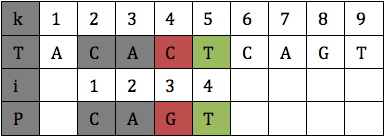
\includegraphics[scale=0.4]{BadCharStep1.png}
	\label{fig:BadChar1}}
\quad
	\subfigure[Ocurre un fallo en $k=7$]{%
	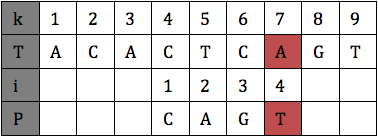
\includegraphics[scale=0.4]{BadCharStep2.png}
	\label{fig:BadChar2}}
\quad
	\subfigure[Se encuentra una ocurrencia de {\it p}]{%
	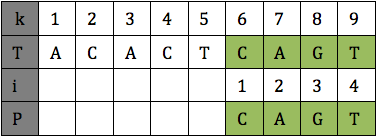
\includegraphics[scale=0.4]{BadCharStep3.png}
	\label{fig:BadChar3}}
\caption[Ejemplo de aplicación de la regla del carácter malo]{Ejemplo de aplicación de la regla del carácter malo}
\label{fig:BadChar}
\end{figure}
\end{example*}
\myrule{}{}
\subsubsection{Regla fuerte del sufijo bueno}
La regla del prefijo malo es útil cuando tenemos alfabetos extensos o se aplica en ambientes donde es altamente probable que ocurran fallos. Para los casos en que se tiene una probabilidad alta de fallo en posiciones finales de un patrón es útil la regla del sufijo bueno.\\
Supongamos que se comparan con éxito los últimos $t$ caracteres de {\it p} (de derecha a izquierda), pero el siguiente carácter falla. Sea $y$ el carácter de {\it p} en la posición $m – \mid t \mid - 1$ según {\it p} y el carácter $x$ de {\it T} alineado a $y$ tal que $x \not= y$.
En estas condiciones la \emph{regla del sufijo bueno} busca la secuencia $t’$ de {\it p} más a la derecha que cumpla que sea idéntica a $t$, que no sea sufijo de {\it p} y que además, $z$, el carácter inmediatamente a la izquierda de $t’$ sea distinto a $y$. Esta situación se ilustra en la figura \ref{fig:goodSufix1}.
\begin{figure}[H]
	\centering
		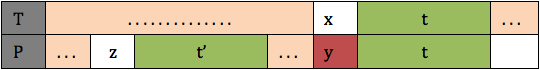
\includegraphics[scale=0.5]{GoodSufix1.png}
		\rule{35em}{0.5pt}
	\caption[Regla del sufijo bueno]{Regla del sufijo bueno}
	\label{fig:goodSufix1}
\end{figure}
Si no existe $t'$ pero existe $t''$ tal que $t''$ es sufijo de $t$ y existe una ocurrencia de $t''$ prefijo de $p$, se debe desplazar $p$ de forma tal que se logre la alineación entre $t''$ de $p$ y $t''$ de {\it T}. Este caso abarca el hecho de encontrar una ocurrencia de $p$ en el texto. En caso que $t''$ sea vacía, se debe desplazar $p$ $m$ posiciones hacia la derecha.\\
Formalizaremos los conceptos anteriormente explicados definiendo dos funciones $L'$ y $l'$.\\
Para cada índice $i=2..m$ de {\it p} se define $L'(i)$ como el máximo $j$, $j<m$, tal que $p[i,m]$ es sufijo de $p[1,j]$ y $p[i-1]$ no coincide con el carácter precedente del sufijo (es decir el carácter $p[j - \mid p[i,m] \mid]$).
Por último definimos $l’(i)$, $i > 1$, como la cantidad de caracteres del sufijo más largo de $p[i,n]$ que también es prefijo de {\it p}. De no existir dicho valor definimos  $l’(i)=0$.
\begin{example*}
Considerando $p=catgatgat$ tenemos que $L'(8)=3$ (Notar que $L'(8)\not=6$ porque $p[4]= p[i-1]=p[7]$), mientras que, para todo $1 \leq i \leq 10$, $l'(i)=0$.
\end{example*}
\myrule{}{}
Al procesar el texto se puede utilizar la regla del sufijo bueno cuando ocurre un fallo en la posición $i-1$ de $p$ de la siguiente forma:
\begin{itemize}
\item Si $L'(i) > 0$ se debe desplazar el patrón $p$ $(m - L'(i))$ posiciones hacia la derecha (esta situación es la presentada en la figura \ref{fig:goodSufix1}).
\item Si $L'(i) = 0$ ($t'$ es vacía) se debe deslpazar el patrón $p$ $(m - l'(i))$ posiciones hacia la derecha .
\end{itemize}
Si ocurre un fallo al comparar la posición {\it m-esíma} (primera comparación) se debe desplazar $p$ una posición a la derecha.
Al encontrar una ocurrencia del patrón $p$, se desplaza $p$ $(m - l(2)')$ posiciones hacia la derecha.
\section{Algoritmos de búsqueda exacta de múltiples patrones en un texto}
Dado un conjunto de patrones $P=\{p_{1}...p_{k}\}$, los algoritmos de búsqueda exacta de múltiples patrones en un texto hallan las ocurrencias de cada patrón de $P$ dentro de un texto.
Los algoritmos de este tipo que presentaremos en este documento se basan en las estructuras de datos {\it trie} y {\it árbol de sufijos} detalladas en las secciones \ref{sec:deftrie} y \ref{sec:defSufixTree} respectivamente.\\
Cabe notar que el algoritmo de Aho Corasick (capítulo \ref{Chapter2}) y MSW (capítulo \ref{Chapter3}) caen dentro de esta categoría, siendo el primero una solución clásica a este problema.
\subsection{Árbol de prefijos o Trie}
\label{sec:deftrie}
Definimos $\mathcal{T}$ como un \emph{trie} o árbol de prefijos de un conjunto de patrones {\emph P} sobre un alfabeto {\it A} si $\mathcal{T}$ es un árbol con raíz que cumple las siguientes propiedades \cite{GUS}:
\begin{itemize}
\item Cada arista de $\mathcal{T}$ se etiqueta con un único símbolo del alfabeto {\it A}.
\item Para todo par de aristas salientes de un nodo de $\mathcal{T}$ se cumple que sus etiquetas son diferentes.
\item Por cada patrón $p \in {\it P}$ existe un nodo {\it v} en $\mathcal{T}$ tal que la secuencia de caracteres resultantes de la concatenación de todos los símbolos en el camino desde el nodo raíz hasta el nodo {\it v} es igual a $p$.
\item La secuencia de caracteres que resulta de concatenar las etiquetas del camino desde el nodo raíz hasta cualquier hoja de $\mathcal{T}$ es un patrón que se encuentra en {\emph P}.
\end{itemize}
\begin{example*}
\label{ex:example1}
Sea \emph{P} un conjunto de patrones sobre un alfabeto \{a, c, g, t\} tal que \emph {P} = \{cg, acg, act, acta, cgg\}, la estructura {\it trie} resultante es la presentada en la figura \ref{fig:trie}. 
\begin{figure}[H]
\centering

\begin{tikzpicture}[every tree node/.style={draw,circle},fill=blue!20,
   level distance=1.75cm,sibling distance=0.8cm, 
   edge from parent path={(\tikzparentnode) -- (\tikzchildnode)}]
\Tree [.\node[fill=blue!20] {}; 
	\edge node[left] {a};  
    [.\node[fill=blue!20] {}; 
      \edge node[left] {c};  
      [.\node[fill=blue!20] {}; 
		   \edge node[left] {g};  
		   [.\node[fill=blue!20] {}; ] 
		   \edge node[right] {t};
	       [.\node[fill=blue!20] {}; 
	     	  \edge node[right] {a};
	     	  [.\node[fill=blue!20] {}; ] 
    		   ]
       ]
    ]
    	\edge node[right] {cg};  
    [.\node[fill=blue!20] {}; 
      \edge node[right] {g};
       [.\node[fill=blue!20] {}; ]
    ]
    ];
\end{tikzpicture}
\caption[Ejemplo: trie]{{\it trie}}
	\label{fig:trie}
\end{figure}
\end{example*}
\myrule{}{}
A continuación introducimos un conjunto de definiciones que aplican a un árbol $\mathcal{T}$ y alfabeto {\it A}, estas definiciones serán usadas a lo largo de todo este documento.
\begin{itemize}
\item Se define \emph{camino} en un árbol como cualquier secuencia de nodos $n_{1}...n_{k}$ que cumpla que cada nodo es padre del siguiente en la secuencia. La \emph{longitud} del camino se define como el número de arístas que se recorren, es decir el número de nodos de la secuencia menos uno ($k - 1$).
\item La \emph{profundidad de un nodo} se define como la longitud del camino que comienza en la raíz y termina en el nodo. La profundidad de la raíz es cero.
\item Asociamos a cada arista de $\mathcal{T}$ una secuencia de caracteres de {\it A} que llamaremos \emph{etiqueta} de la arista. En un trie, todas las aristas tienen etiquetas de largo 1.
\item Llamaremos \emph{etiqueta de un nodo} {\it v} (denotada $L(v)$) a la concatenación de las etiquetas de las aristas que se encuentran en el camino definido entre la raíz de $\mathcal{T}$ y {\it v}.
\item Si hay un camino del nodo {\it u} al nodo {\it v}, {\it u} es \emph{ascendiente} de {\it v} y {\it v} es \emph{descendiente} de {\it u}. Esta situación la notaremos como $v \prec u$
\end{itemize}
Esta estructura de datos sirve de base para el algoritmo de Aho Corasick (capítulo \ref{Chapter2}) y para resolver otro tipo de problemas de búsqueda en un texto. Por ejemplo, esta estructura puede ser utilizada para resolver el problema del diccionario ({\it dictionary problem}). En este problema un conjunto de patrones es insertado en un {\it Trie}, luego, se verifica si secuencias individuales de un texto pertenecen o no al diccionario (conjunto de patrones).
\subsection{Árbol de sufijos}
\label{sec:defSufixTree}
Un árbol de sufijos $\mathcal{T}$ para una secuencia de caracteres $s[1,m]$, en un alfabeto {\it A}, es un árbol con raíz que cumple las siguientes propiedades \cite{GUS}:
\begin{itemize}
\item El árbol tiene exactamente $m$ hojas.
\item Cada nodo interno tiene al menos dos nodos descendientes, salvo, potencialmente, el nodo raíz.
\item Cada arista se etiqueta con una cadena de caracteres no vacía.
\item Dado un nodo $v$ del árbol, no existen dos aristas salientes de $v$ que coincidan en el primer carácter de sus etiquetas.
\item Cada hoja $v$ de $\mathcal{T}$ cumple que $L(v)$ es un sufijo de $s$.
\end{itemize}
\begin{example*}
En la figura \ref{fig:sufixTree1} se presenta un árbol de sufijos construido a partir de $s=tactag$
\begin{figure}[H]
\centering

\begin{tikzpicture}[every tree node/.style={draw,circle},fill=blue!20,
   level distance=1.75cm,sibling distance=0.8cm, 
   edge from parent path={(\tikzparentnode) -- (\tikzchildnode)}]
\Tree [.\node[fill=blue!20] {}; 
	\edge node[left] {a};  
    [.\node[fill=blue!20] {}; 
      \edge node[left] {ctag};  
      [.\node[fill=blue!20] {};  ]
      \edge node[right] {g};
       [.\node[fill=blue!20] {}; ]
    ]
    \edge node[left] {ctag};
    [.\node[fill=blue!20] {};]
    \edge node[right] {g};
    [.\node[fill=blue!20] {};]
    	\edge node[right] {ta};  
    [.\node[fill=blue!20] {}; 
      \edge node[left] {ctag};  
      [.\node[fill=blue!20] {};  ]
      \edge node[right] {g};
       [.\node[fill=blue!20] {}; ]
    ]
    ];
\end{tikzpicture}
\caption[Ejemplo: Árbol de sufijos]{Árbol de sufijos construído a partir de $s=tactag$}
	\label{fig:sufixTree1}
\end{figure}
\end{example*}
\myrule{}{}
Estos árboles pueden ser representados de forma compacta, etiquetando las aristas con el índice inicial y final. Esto es, cada arista etiquetada con una sub secuencia $s[i,j]$ es representada mediante los índices $i$ y $j$. Por ejemplo, tomando $s=tactag$, la arista etiquetada por $ctag$ queda representada por $(3,6)$.\\
Si un sufijo $w$ de $s$ es prefijo de otro sufijo $s$ no se podrá construir un árbol de sufijos a partir de $s$ ya que el nodo correspondiente a $L(w)$ no será una hoja. Por ejemplo, si consideramos $s=tagcag$, no se puede construir un árbol de sufijos con la definición anteriormente dada ya que el sufijo $w=ag$ es prefijo del también sufijo $agcag$. Para evitar este problema podemos agregar al final de $s$ un carácter especial $\$$ no perteneciente a {\it A}.\\
El algoritmo de Ukkonen \cite{UK95} o el algoritmo de Weiner \cite{WEINER} permiten construir un árbol de sufijos partiendo de una secuencia de caracteres $s$, $\mid s \mid =n$, en tiempo $O(n)$.\\
Esta estructura de datos nos permite buscar un patrón $p$, $\mid p \mid = m$, dentro de un texto en un tiempo $O(n+m)$. Para ello se construye el árbol de sufijos de texto {\it T} y luego se comparan los caracteres de $p$ comenzando del nodo raíz y descendiendo por las aristas del árbol que coincidan con $p$. Si es posible encontrar una coincidencia completa de $p$ existirán $z$ hojas debajo del camino recorrido, cada una de ellas es el comienzo de una ocurrencia de $p$. Si no es posible encontrar una coincidencia completa de $p$ en el árbol no se habrá encontrado ninguna ocurrencia del patrón en el texto.\\
El árbol de sufijos se puede generalizar de forma tal que se inserten sobre un mismo árbol de sufijos un conjunto de múltiples secuencias de caracteres $S=\{s_{1}..s_{k}\}$.\\
La estrategia de construcción más simple de este árbol de sufijos generalizado es concatenar todas las secuencias de forma tal que se defina una nueva secuencia $c=s_{1}\$_{1}..s_{k}\$_{k}$ donde $\$_{i}$ no pertenece al alfabeto y representa una marca única que identifica la finalización de una secuencia $s_{i}$. Luego se crea un árbol de sufijos partiendo de $c$, etiquetando a cada hoja con una tupla $(i,j)$, donde $i$ identifica la secuencia y $j$ el índice de comienzo de la secuencia $s_{i}$.\\
Otra forma de construir este árbol es agregar una a una las secuencias de $S$, utilizando de forma incremental el algoritmo de Ukkonen.
